\documentclass[acmlarge,11pt]{acmart}
\usepackage{minted}
\usepackage{tikz}
\usetikzlibrary{automata, positioning, arrows}
\tikzset{->,  % makes the edges directed
>=stealth, % makes the arrow heads bold
node distance=3cm, % specifies the minimum distance between two nodes. Change if necessary.
every state/.style={thick, fill=gray!10}, % sets the properties for each ’state’ node
initial text=$ $, % sets the text that appears on the start arrow
}

% Remove DOI info
\makeatletter
\renewcommand\@formatdoi[1]{\ignorespaces}
\makeatother

\settopmatter{printacmref=false} % Removes citation information below abstract
\renewcommand\footnotetextcopyrightpermission[1]{} % removes footnote with conference information in first column
\pagestyle{empty} % removes running headers

\AtBeginDocument{%
  \providecommand\BibTeX{{%
    \normalfont B\kern-0.5em{\scshape i\kern-0.25em b}\kern-0.8em\TeX}}}

\setcopyright{none}

\fancyfoot{}

\begin{document}
\title{DRILLS: Debugging RTL Intelligently with Localization from Long-Simulation}
\author{Vighnesh Iyer}
\email{vighnesh.iyer@berkeley.edu}
\author{Donggyu Kim}
\email{dgkim@berkeley.edu}
\affiliation{
  \institution{UC Berkeley}
}
\renewcommand{\shortauthors}{Iyer and Kim}

\begin{abstract}
  With increasing RTL design complexity it is increasingly difficult to debug why a subset of tests fail in chip-level emulation.
  We propose the use of specification mining to 
  % TODO TODO TODO TODO
  %Commonly, realistic workloads are run on RTL being emulated on an FPGA and
  %from the use of powerful DSLs (Chisel) and higher levels of abstraction (HLS), the number of subtle bugs present in a design also increases.
  %Many design bugs are difficult to catch with unit testing...
  %As hardware complexity increases to meet performance targets and implement required functionality, verification becomes much more challenging. A recent study shows that verification dominates time-to-market and it is getting worse over time\supercite{Foster}. Therefore, it is critical to invent effective hardware verification tools to alleviate time and manual effort to trace the root cause of a design bug.
\end{abstract}
\maketitle
\thispagestyle{empty}
\section{Introduction}
Specification mining is a technique to extract LTL properties from a set of traces of signals.
This technique can be applied for several purposes in the domain of digital hardware verification including:
\begin{enumerate}
  \item Developing a suite of assertions to be used for design regressions: once a design is mature, most of the interface boundary specifications are well defined and fine-grained assertions derived from specification mining can help catch regressions when design refinements or optimizations are being made.
  \item A starting point for formally specifying a design: once a design can pass random-stimulus based and directed unit tests, specification mining can be used to extract properties that have been consistently observed in the test waveforms. These properties can then be used as assertions to prove formally.
  \item Early anomaly detection and localization on long-running tests on mature RTL: if a specific test fails on an RTL design while many other tests pass, specification mining can reveal \textit{where and when} a failing test begins to produce unusual behavior in the RTL, guiding the designer to the bug location.
\end{enumerate}
In this report, we will focus on applying specification mining to address the last point above.

\subsection{Motivation}
RTL designs are increasing in complexity and are thus more prone to having subtle bugs that are not caught in regular verification flows. Typical techniques such as randomized-stimulus testing, directed testing, and fuzz testing have a difficult time catching bugs that require the RTL be put into a very specific state.

These subtle bugs are usually caught when performing chip emulation or FPGA prototyping when running realistic workloads on the RTL.
Real workloads usually involve traces that are billion of cycles long, and are thus too slow to perform using RTL simulation which provides full design visibility.
DESSERT\cite{Kim_2018} demonstrates a technique to capture full-visibility waveform traces from fast running FPGA simulation.
Using DESSERT, an out-of-order RISC-V processor (BOOM\cite{Celio_2015}) is deterministically emulated on an FPGA with runtime assertion monitors while running the SPEC2017 benchmark suite.
During the execution of several tests, synthesized assertions were violated which revealed there exists some subtle bugs in the core causing some benchmarks to fail.

While these assertions are useful for catching errors, they are very high-level and don't direct the designer to where a bug originated.
As an example, the "\texttt{Pipeline has hung}" assertion (in BOOM) is generated with the following Chisel code:

\begin{minted}[fontsize=\small]{scala}
// detect pipeline freezes and throw error
val idle_cycles = freechips.rocketchip.util.WideCounter(32)
when (rob.io.commit.valids.asUInt.orR ||
      csr.io.csr_stall ||
      io.rocc.busy ||
      reset.asBool) {
  idle_cycles := 0.U
}
assert (!(idle_cycles.value(13)), "Pipeline has hung.")
\end{minted}

In words, this says, "If there is a good reason to stall the pipeline, reset \texttt{idle\_cycles}, otherwise let it tick up to 13 before declaring something has gone wrong."
This assertion does not give any insight as to what bad event happened, or when and where it happened.
Since these assertions are thrown after billions of cycles it is possible that some $\mu$-arch state was corrupted early in the simulation and only triggered this assertion much later during execution.
DESSERT enables extracting waveforms for a variable number of cycles before the assertion triggers, but even with the waveform dumps in hand, the designer was unable to localize the bug.
Our aim in developing this specification mining tool is to hunt out the locations of these trickly bugs in BOOM and fix them.

\subsection{Hypothesis}
Mature RTL designs (like BOOM) pass almost all tests run on them, including a full set of ISA tests, a boot of Linux, and real applications running on an OS.
If a test fails on a mature design, we hypothesize that an \textit{assumption} the designer made about the RTL was violated somewhere and at some time during the failing test execution, that was not violated on any successful test execution.
These assumptions can include believing that a certain register cannot hold certain values or higher-level properties such as: "the memory system will respond to my request within 5 cycles".

We believe specification mining can be used to extract designer assumptions about the RTL design by mining fine-grained LTL properties on waveforms of successful test executions.
These mined properties can be added to the RTL design as assertions and replaying the failing test should cause a violation of a mined property.
These violations can be used to catch a faulty assumption \textit{earlier and with greater locality} than the high-level assertions originally present in the design.

\subsection{Problem Definition}
\par
\textbf{Given}:
\begin{itemize}
  \item An RTL design driven with only one global clock
  \item A large set of VCD (value change dump) files produced when running a full suite of tests in an RTL simulator
  \item One or just a few failing tests in the suite characterized by a failed high-level assertion, hanging/global timeout, or a bad exit code
\end{itemize}
\textbf{Produce}:
\begin{itemize}
  \item A set of mined LTL properties involving signals (combinational nets and registers) of the RTL design that aren't violated on any passing test
  \item A method of ranking the mined LTL properties
  \item A program that can check a VCD against the mined properties to find any violations for that execution trace
\end{itemize}

\section{Approach}
Our plan is to first create the products above with a small RTL design.
We use \texttt{riscv-mini}\cite{riscv-mini}, a simple 3-stage in-order RISC-V processor as the RTL we will use to test the specification mining engine.
\texttt{riscv-mini} has real instruction and data caches and implements the RV32UI ISA subset which is capable of running the entire \texttt{riscv-tests}\cite{riscv-tests} test suite.
The test suite contains a comprehensive set of ISA tests and benchmarks which will be used to generate the VCD files for mining.

\subsection{Prior Work}
Specification mining has been applied to both software and hardware verification.
% TODO TODO TODO TODO
% Mention Texada and Sanjit's Toyota paper
% Mention Wenchao Li's thesis as the main inspiration
% Mention SAT-based mux methods for bug localization and point out its shortcomings

\subsection{High-Level Flow}
The long-term plan is to leverage the spec mining engine and the prior work of DESSERT to provide an FPGA-acclererated debugging platform.
We plan to take waveforms of successful test executions from RTL simulation and FPGA emulation of BOOM and feed the spec mining engine to infer LTL properties.
The buggy RTL is instrumented by taking the LTL properties and converting them to property monitor FSMs which are stiched into the original design.
The assertions are synthesized for FPGA emulation using the same methodology described in DESSERT, and the failing tests are executed.
It is our hope that the failing tests will trigger failures in the mined properties before the failure becomes visible to the user (via a high-level assertion violation, hanging/timout, or a bad exit code).
\begin{figure}[H]
  \centering
  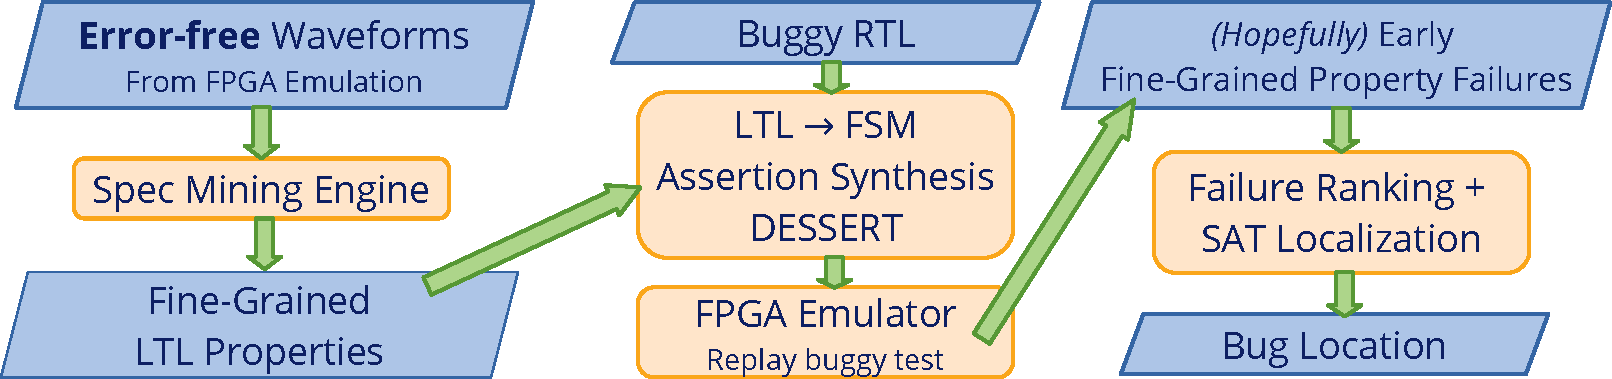
\includegraphics[width=0.8\textwidth]{figs/proposed_approach.pdf}
  \caption{The proposed tool flow to use specification mining and FPGA-accelerated simulation to pinpoint bug locations in for an RTL design .}
  \label{fig:proposed_approach}
\end{figure}
The mined properties which were violated can be ranked based on the time of their violation and we can use the SAT localization techniques mentioned above to further pinpoint the bug location.

\section{Model and Algorithms}
In this section, we will specify the formal model for LTL specification mining, how we adapted LTL formulas for RTL, and the algorithms used in the spec mining engine.

\subsection{Hardware Idioms in LTL}
They can be used to describe many common idioms present in RTL. A few examples:
\begin{itemize}
  \item There should eventually be a response (\texttt{resp}) after a request (\texttt{req}) \\
    $\quad \mathbf{G}\, (\mathtt{req} \rightarrow \mathbf{XF}\, \mathtt{resp})$
  \item There should be a response in 2 cycles after a request \\
    $\quad \mathbf{G}\, (\mathtt{req} \rightarrow \mathbf{XX}\, \mathtt{resp})$
  \item The ready/valid interface should keep \texttt{valid} high once it has been asserted until \texttt{ready} goes high \\
    $\quad \mathbf{G}\, (\mathtt{valid} \rightarrow \mathbf{X}\, (\mathtt{valid}\, \mathbf{U}\, \mathtt{ready}))$
  \item After a ready/valid transaction, the slave should be \texttt{ready} again within 2 cycles \\
    $\quad \mathbf{G}\, ((\mathtt{valid} \land \mathtt{ready}) \rightarrow (\mathbf{X}\, \mathtt{ready} \lor \mathbf{XX}\, \mathtt{ready}))$
\end{itemize}

\subsubsection{LTL Templates} \label{templates}
The formulas above can be templated by replacing the concrete signals (such as \texttt{ready}, \texttt{resp}, etc.) with variable placeholders. We consider 4 LTL templates for spec mining derived from Li's prior work\cite{Li_2014}:

\begin{itemize}
  \item Alternating: $a\, \mathbf{A}\, b$
  \item Until: $\mathbf{G}\, (a \rightarrow \mathbf{X}\, (a\, \mathbf{U}\, b))$
  \item Next: $\mathbf{G}\, (a \rightarrow \mathbf{X}\, b)$
  \item Eventual: $\mathbf{G}\, (a \rightarrow \mathbf{X F}\, b)$
\end{itemize}

where $a$ and $b$ are some boolean expressions derived from the signals in the RTL.

\subsection{Adapting LTL Templates for RTL}
RTL simulations produce a set of finite-length traces of bitvectors.
In contrast, LTL properties are defined over infinite-length traces of atomic propositions.
We convert bitvector traces to traces of \textit{delta events} which are treated as atomic propositions, and we employ notions of \textit{falsifiability} and \textit{support} to mine LTL properties on finite length traces.

Let a signal trace $\tau_i$ be a tuple of length $T$ which contains the value of the signal $i$ (a bitvector) at every discrete timestep of an RTL simulation.
Let there be $N$ signals in the RTL design: $i \in [0,N)$.
We can convert $\tau_i$ to its delta trace $\tau_{\Delta i}$ as such:
\begin{align*}
  \tau_{\Delta i}(t) = (\tau_i(t-1) \neq \tau_i(t)) \quad \forall t \in [1,T)
\end{align*}

Note that $\tau_{\Delta i}$ is a tuple of length $T-1$ and is a trace of atomic propositions.
Simply put, we convert a bitvector signal trace to a boolean trace which is 1 whenever the signal changes value, and 0 otherwise.
We now consider the templates in section \ref{templates} in the context where $a, b = \tau_{\Delta i}, \tau_{\Delta j}, i \neq j$, for some $i, j$.

Here is a concrete example where $k, q$ are bitvector signals in an RTL design where $k$ is 1 bit wide and $q$ is 10 bits wide:
\begin{align*}
  \tau_{k} &= (0, 1, 1, 1, 0) \\
  \tau_{q} &= (0, 0, 200, 200, 300) \\
  \tau_{\Delta k} &= (1, 0, 0, 1) \\
  \tau_{\Delta q} &= (0, 1, 0, 1)
\end{align*}

Note that even though $k$ is a boolean signal and can already be treated as an atomic proposition, we only mine LTL properties on its \textit{delta trace} and not the signal itself.

In RTL designs, it is usually the case that the density of transitions for a given signal is fairly low.
Signal traces can be stored in a compressed format where we only record the timestep in which the signal value changes.
Indeed, this is conveniently how traces are stored in a VCD (value change dump) file which is the input to the spec miner.
We can extract sparsely represented delta traces from a VCD file as a tuple of timesteps where the signal transitions. %of tuples where the inner tuple consists of (timestep, value) pairs.
\begin{align*}
  \tau_{\Delta k, compressed} &= (0, 3) \\
  \tau_{\Delta q, compressed} &= (1, 3)
\end{align*}

We want to consider the templates in section \ref{templates}, so we can zip 2 compressed delta traces together that indicates which of the signals transitioned.
\begin{align*}
  \tau_{\Delta k, \Delta q} &= ((\Delta k, \lnot \Delta q), (\lnot \Delta k, \Delta q), (\Delta k, \Delta q))
\end{align*}
This means that initially, $k$ transitioned and $q$ did not on a given timestep, then on a future timestep $q$ transitioned and $k$ did not, and on another future timestep both $k$ and $q$ transitioned.
Note that in this data structure, it is impossible to have a tuple where both $k$ and $q$ \textit{did not} transition.
This data structure is perfect to construct automatons that mine LTL properties.


\subsection{Mining with Automata}
We construct FSMs for each of the LTL property templates that take zipped compressed delta traces as an input.

\subsubsection{Falsifiability and Support}
A given LTL property template is \textit{falsifiable} over a zipped delta trace if its mining automaton reaches a state from which it can move to the \textit{falsified} state in one step.
We loosely define the \textit{support} for an LTL property over a trace as the number of times the pattern "repeats".
It will be made explicit in the FSMs for each LTL template as to when a pattern "repetition" occurs; we have yet to formalize this notion.
We will abbreviate falsifiable as $f$ and support as $s$.

\subsubsection{Alternating}
\begin{figure}[H]
  \centering
  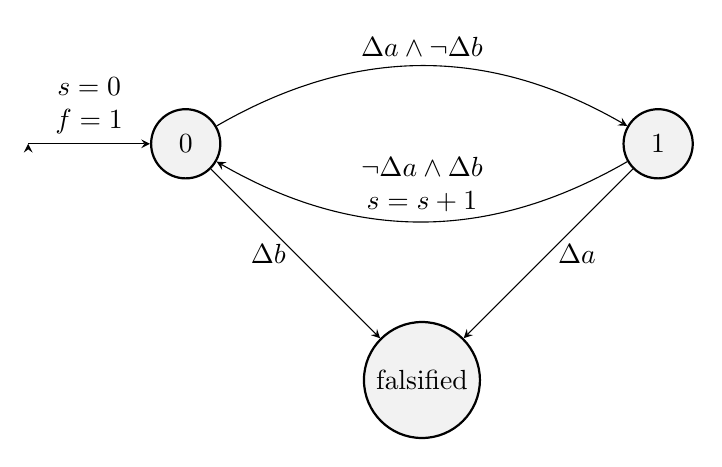
\begin{tikzpicture}
    \node[state] (q1) at (0,0) {0};
    \node[state] (q2) at (6,0) {1};
    \node[state] (q3) at (3,-3) {falsified};
    \draw (-2,0) edge[above] node[align=center]{$s = 0$\\$f = 1$} (q1)
    (q1) edge[bend left, above] node{$\Delta a \land \lnot \Delta b$} (q2)
    (q2) edge[bend left, above] node[align=center]{$\lnot \Delta a \land \Delta b$\\$s = s + 1$} (q1)
    (q1) edge[left] node{$\Delta b$} (q3)
    (q2) edge[right] node{$\Delta a$} (q3);
  \end{tikzpicture}
\caption{Automaton that mines the alternating LTL pattern}
\label{fig:alternating}
\end{figure}

The automaton in figure \ref{fig:alternating} mines the alternating pattern and advances support when a $\Delta a$ then $\Delta b$ sequence occurs.
This pattern is violated if $\Delta a$ and $\Delta b$ are both true on the same timestep.

\subsubsection{Until}
\begin{figure}[H]
  \centering
  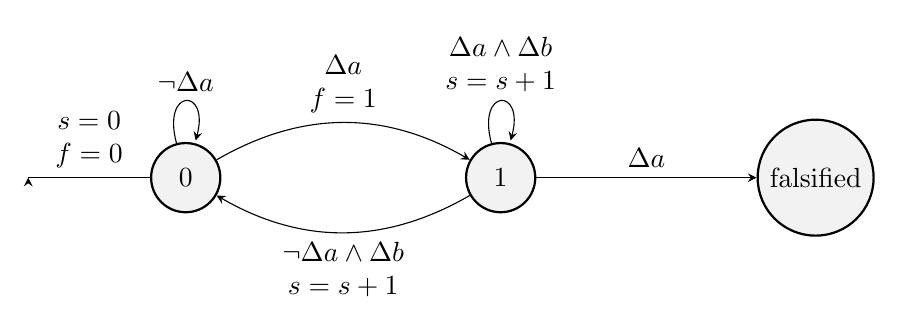
\begin{tikzpicture}
    \node[state] (q1) at (0,0) {0};
    \node[state] (q2) at (4,0) {1};
    \node[state] (q3) at (8,0) {falsified};
    \draw (-2,0) edge[above,-] node[align=center]{$s = 0$\\$f = 0$} (q1)
    (q1) edge[loop above] node{$\lnot \Delta a$} (q1)
    (q1) edge[bend left, above] node[align=center]{$\Delta a$\\$f = 1$} (q2)
    (q2) edge[bend left, below] node[align=center]{$\lnot \Delta a \land \Delta b$\\$s = s + 1$} (q1)
    (q2) edge[loop above] node[align=center]{$\Delta a \land \Delta b$\\$s = s + 1$} (q2)
    (q2) edge[above] node{$\Delta a$} (q3);
  \end{tikzpicture}
\caption{Automaton that mines the until LTL pattern}
\label{fig:until}
\end{figure}

The automaton in figure \ref{fig:until} mines the until pattern. If $\Delta a$ is seen 2 times in a row without a $\Delta b$ then this pattern is falsified. Note that if $\Delta a$ never occurs, this pattern can't be falsifiable on that particular delta trace.

\subsubsection{Next}
\begin{figure}[H]
  \centering
  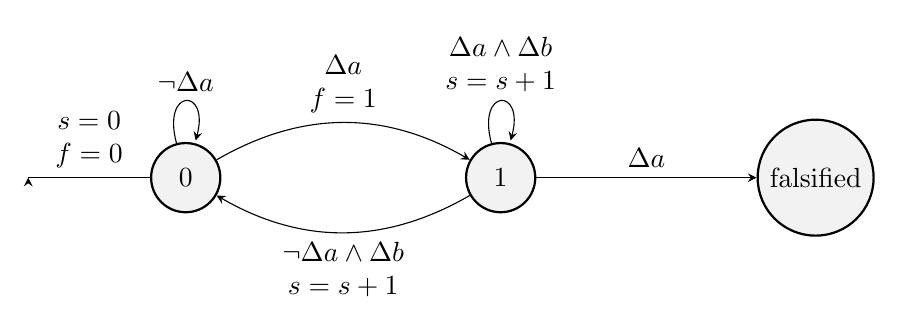
\begin{tikzpicture}
    \node[state] (q1) at (0,0) {0};
    \node[state] (q2) at (4,0) {1};
    \node[state] (q3) at (8,0) {falsified};
    \draw (-2,0) edge[above,-] node[align=center]{$s = 0$\\$f = 0$} (q1)
    (q1) edge[loop above] node{$\lnot \Delta a$} (q1)
    (q1) edge[bend left, above] node[align=center]{$\Delta a$\\$f = 1$} (q2)
    (q2) edge[bend left, below] node[align=center]{$\lnot \Delta a \land \Delta b$\\$s = s + 1$} (q1)
    (q2) edge[loop above] node[align=center]{$\Delta a \land \Delta b$\\$s = s + 1$} (q2)
    (q2) edge[above] node{$\Delta a$} (q3);
  \end{tikzpicture}
\caption{Automaton that mines the next LTL pattern}
\label{fig:next}
\end{figure}


\subsection{Merging Properties}

\subsection{Checking Against VCDs}

\subsection{Challenges}

\section{Results}

\subsection{Future Work}
% Additional templates
% Faster miner (software engineering)
% Custom ways to construct AP traces from signal traces (ready/valid boundary, using boolean signals directly, etc.)
% General miner (take any LTL formula and construct a miner automatically)
% 

\section{Course-Related}

\subsection{Roles}

\subsection{Usage of Class Topics}

\subsection{Feedback}


Journals use one of three template styles. All but three ACM journals
use the {\verb|acmsmall|} template style:
\begin{itemize}
\item {\verb|acmsmall|}: The default journal template style.
\item {\verb|acmlarge|}: Used by JOCCH and TAP.
\item {\verb|acmtog|}: Used by TOG.
\end{itemize}

The majority of conference proceedings documentation will use the {\verb|acmconf|} template style.
\begin{itemize}
\item {\verb|acmconf|}: The default proceedings template style.
\item{\verb|sigchi|}: Used for SIGCHI conference articles.
\item{\verb|sigchi-a|}: Used for SIGCHI ``Extended Abstract'' articles.
\item{\verb|sigplan|}: Used for SIGPLAN conference articles.
\end{itemize}

\subsection{Template Parameters}

In addition to specifying the {\itshape template style} to be used in
formatting your work, there are a number of {\itshape template parameters}
which modify some part of the applied template style. A complete list
of these parameters can be found in the {\itshape \LaTeX\ User's Guide.}

Frequently-used parameters, or combinations of parameters, include:
\begin{itemize}
\item {\verb|anonymous,review|}: Suitable for a ``double-blind''
  conference submission. Anonymizes the work and includes line
  numbers. Use with the \verb|\acmSubmissionID| command to print the
  submission's unique ID on each page of the work.
\item{\verb|authorversion|}: Produces a version of the work suitable
  for posting by the author.
\item{\verb|screen|}: Produces colored hyperlinks.
\end{itemize}

This document uses the following string as the first command in the
source file:
\verb|\documentclass[sigconf]{acmart}|.

\section{Modifications}

Modifying the template --- including but not limited to: adjusting
margins, typeface sizes, line spacing, paragraph and list definitions,
and the use of the \verb|\vspace| command to manually adjust the
vertical spacing between elements of your work --- is not allowed.

{\bfseries Your document will be returned to you for revision if
  modifications are discovered.}

\section{Typefaces}

The ``\verb|acmart|'' document class requires the use of the
``Libertine'' typeface family. Your \TeX\ installation should include
this set of packages. Please do not substitute other typefaces. The
``\verb|lmodern|'' and ``\verb|ltimes|'' packages should not be used,
as they will override the built-in typeface families.

\section{Title Information}

The title of your work should use capital letters appropriately -
\url{https://capitalizemytitle.com/} has useful rules for
capitalization. Use the {\verb|title|} command to define the title of
your work. If your work has a subtitle, define it with the
{\verb|subtitle|} command.  Do not insert line breaks in your title.

If your title is lengthy, you must define a short version to be used
in the page headers, to prevent overlapping text. The \verb|title|
command has a ``short title'' parameter:
\begin{verbatim}
  \title[short title]{full title}
\end{verbatim}

\section{Authors and Affiliations}

Each author must be defined separately for accurate metadata
identification. Multiple authors may share one affiliation. Authors'
names should not be abbreviated; use full first names wherever
possible. Include authors' e-mail addresses whenever possible.

Grouping authors' names or e-mail addresses, or providing an ``e-mail
alias,'' as shown below, is not acceptable:
\begin{verbatim}
  \author{Brooke Aster, David Mehldau}
  \email{dave,judy,steve@university.edu}
  \email{firstname.lastname@phillips.org}
\end{verbatim}

The \verb|authornote| and \verb|authornotemark| commands allow a note
to apply to multiple authors --- for example, if the first two authors
of an article contributed equally to the work.

If your author list is lengthy, you must define a shortened version of
the list of authors to be used in the page headers, to prevent
overlapping text. The following command should be placed just after
the last \verb|\author{}| definition:
\begin{verbatim}
  \renewcommand{\shortauthors}{McCartney, et al.}
\end{verbatim}
Omitting this command will force the use of a concatenated list of all
of the authors' names, which may result in overlapping text in the
page headers.

The article template's documentation, available at
\url{https://www.acm.org/publications/proceedings-template}, has a
complete explanation of these commands and tips for their effective
use.

\section{Rights Information}

Authors of any work published by ACM will need to complete a rights
form. Depending on the kind of work, and the rights management choice
made by the author, this may be copyright transfer, permission,
license, or an OA (open access) agreement.

Regardless of the rights management choice, the author will receive a
copy of the completed rights form once it has been submitted. This
form contains \LaTeX\ commands that must be copied into the source
document. When the document source is compiled, these commands and
their parameters add formatted text to several areas of the final
document:
\begin{itemize}
\item the ``ACM Reference Format'' text on the first page.
\item the ``rights management'' text on the first page.
\item the conference information in the page header(s).
\end{itemize}

Rights information is unique to the work; if you are preparing several
works for an event, make sure to use the correct set of commands with
each of the works.

\section{CCS Concepts and User-Defined Keywords}

Two elements of the ``acmart'' document class provide powerful
taxonomic tools for you to help readers find your work in an online
search.

The ACM Computing Classification System ---
\url{https://www.acm.org/publications/class-2012} --- is a set of
classifiers and concepts that describe the computing
discipline. Authors can select entries from this classification
system, via \url{https://dl.acm.org/ccs/ccs.cfm}, and generate the
commands to be included in the \LaTeX\ source.

User-defined keywords are a comma-separated list of words and phrases
of the authors' choosing, providing a more flexible way of describing
the research being presented.

CCS concepts and user-defined keywords are required for all short- and
full-length articles, and optional for two-page abstracts.

\section{Sectioning Commands}

Your work should use standard \LaTeX\ sectioning commands:
\verb|section|, \verb|subsection|, \verb|subsubsection|, and
\verb|paragraph|. They should be numbered; do not remove the numbering
from the commands.

Simulating a sectioning command by setting the first word or words of
a paragraph in boldface or italicized text is {\bfseries not allowed.}

\section{Tables}

The ``\verb|acmart|'' document class includes the ``\verb|booktabs|''
package --- \url{https://ctan.org/pkg/booktabs} --- for preparing
high-quality tables.

Table captions are placed {\itshape above} the table.

Because tables cannot be split across pages, the best placement for
them is typically the top of the page nearest their initial cite.  To
ensure this proper ``floating'' placement of tables, use the
environment \textbf{table} to enclose the table's contents and the
table caption.  The contents of the table itself must go in the
\textbf{tabular} environment, to be aligned properly in rows and
columns, with the desired horizontal and vertical rules.  Again,
detailed instructions on \textbf{tabular} material are found in the
\textit{\LaTeX\ User's Guide}.

Immediately following this sentence is the point at which
Table~\ref{tab:freq} is included in the input file; compare the
placement of the table here with the table in the printed output of
this document.

\begin{table}
  \caption{Frequency of Special Characters}
  \label{tab:freq}
  \begin{tabular}{ccl}
    \toprule
    Non-English or Math&Frequency&Comments\\
    \midrule
    \O & 1 in 1,000& For Swedish names\\
    $\pi$ & 1 in 5& Common in math\\
    \$ & 4 in 5 & Used in business\\
    $\Psi^2_1$ & 1 in 40,000& Unexplained usage\\
  \bottomrule
\end{tabular}
\end{table}

To set a wider table, which takes up the whole width of the page's
live area, use the environment \textbf{table*} to enclose the table's
contents and the table caption.  As with a single-column table, this
wide table will ``float'' to a location deemed more
desirable. Immediately following this sentence is the point at which
Table~\ref{tab:commands} is included in the input file; again, it is
instructive to compare the placement of the table here with the table
in the printed output of this document.

\begin{table*}
  \caption{Some Typical Commands}
  \label{tab:commands}
  \begin{tabular}{ccl}
    \toprule
    Command &A Number & Comments\\
    \midrule
    \texttt{{\char'134}author} & 100& Author \\
    \texttt{{\char'134}table}& 300 & For tables\\
    \texttt{{\char'134}table*}& 400& For wider tables\\
    \bottomrule
  \end{tabular}
\end{table*}

\section{Math Equations}
You may want to display math equations in three distinct styles:
inline, numbered or non-numbered display.  Each of the three are
discussed in the next sections.

\subsection{Inline (In-text) Equations}
A formula that appears in the running text is called an inline or
in-text formula.  It is produced by the \textbf{math} environment,
which can be invoked with the usual
\texttt{{\char'134}begin\,\ldots{\char'134}end} construction or with
the short form \texttt{\$\,\ldots\$}. You can use any of the symbols
and structures, from $\alpha$ to $\omega$, available in
\LaTeX~\cite{Lamport:LaTeX}; this section will simply show a few
examples of in-text equations in context. Notice how this equation:
\begin{math}
  \lim_{n\rightarrow \infty}x=0
\end{math},
set here in in-line math style, looks slightly different when
set in display style.  (See next section).

\subsection{Display Equations}
A numbered display equation---one set off by vertical space from the
text and centered horizontally---is produced by the \textbf{equation}
environment. An unnumbered display equation is produced by the
\textbf{displaymath} environment.

Again, in either environment, you can use any of the symbols and
structures available in \LaTeX\@; this section will just give a couple
of examples of display equations in context.  First, consider the
equation, shown as an inline equation above:
\begin{equation}
  \lim_{n\rightarrow \infty}x=0
\end{equation}
Notice how it is formatted somewhat differently in
the \textbf{displaymath}
environment.  Now, we'll enter an unnumbered equation:
\begin{displaymath}
  \sum_{i=0}^{\infty} x + 1
\end{displaymath}
and follow it with another numbered equation:
\begin{equation}
  \sum_{i=0}^{\infty}x_i=\int_{0}^{\pi+2} f
\end{equation}
just to demonstrate \LaTeX's able handling of numbering.

\section{Figures}

The ``\verb|figure|'' environment should be used for figures. One or
more images can be placed within a figure. If your figure contains
third-party material, you must clearly identify it as such, as shown
in the example below.
\begin{figure}[h]
  \centering
  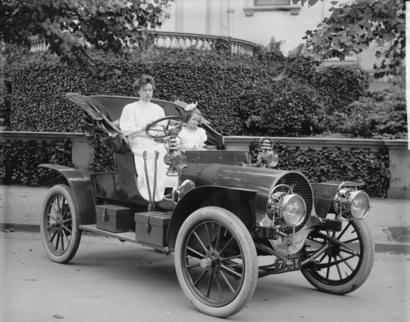
\includegraphics[width=\linewidth]{sample-franklin}
  \caption{1907 Franklin Model D roadster. Photograph by Harris \&
    Ewing, Inc. [Public domain], via Wikimedia
    Commons. (\url{https://goo.gl/VLCRBB}).}
  \Description{The 1907 Franklin Model D roadster.}
\end{figure}

Your figures should contain a caption which describes the figure to
the reader. Figure captions go below the figure. Your figures should
{\bfseries also} include a description suitable for screen readers, to
assist the visually-challenged to better understand your work.

Figure captions are placed {\itshape below} the figure.

\subsection{The ``Teaser Figure''}

A ``teaser figure'' is an image, or set of images in one figure, that
are placed after all author and affiliation information, and before
the body of the article, spanning the page. If you wish to have such a
figure in your article, place the command immediately before the
\verb|\maketitle| command:
\begin{verbatim}
  \begin{teaserfigure}
    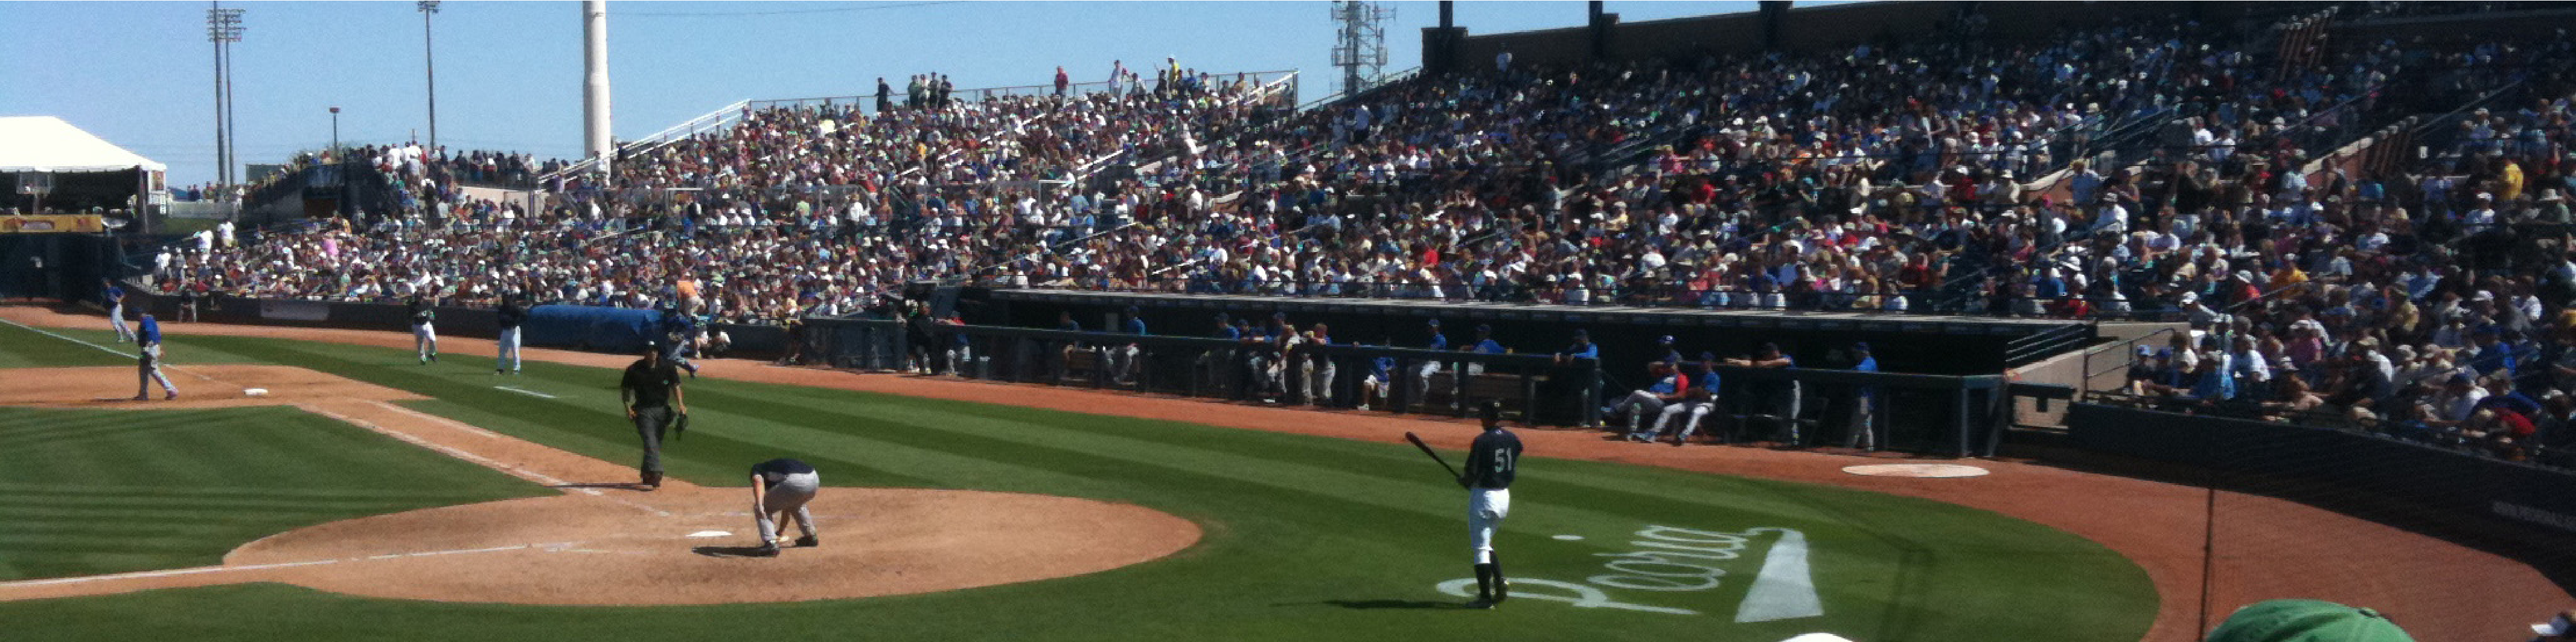
\includegraphics[width=\textwidth]{sampleteaser}
    \caption{figure caption}
    \Description{figure description}
  \end{teaserfigure}
\end{verbatim}

\section{Citations and Bibliographies}

The use of \BibTeX\ for the preparation and formatting of one's
references is strongly recommended. Authors' names should be complete
--- use full first names (``Donald E. Knuth'') not initials
(``D. E. Knuth'') --- and the salient identifying features of a
reference should be included: title, year, volume, number, pages,
article DOI, etc.

The bibliography is included in your source document with these two
commands, placed just before the \verb|\end{document}| command:
\begin{verbatim}
  \bibliographystyle{ACM-Reference-Format}
  \bibliography{bibfile}
\end{verbatim}
where ``\verb|bibfile|'' is the name, without the ``\verb|.bib|''
suffix, of the \BibTeX\ file.

Citations and references are numbered by default. A small number of
ACM publications have citations and references formatted in the
``author year'' style; for these exceptions, please include this
command in the {\bfseries preamble} (before
``\verb|\begin{document}|'') of your \LaTeX\ source:
\begin{verbatim}
  \citestyle{acmauthoryear}
\end{verbatim}

  Some examples.  A paginated journal article \cite{Abril07}, an
  enumerated journal article \cite{Cohen07}, a reference to an entire
  issue \cite{JCohen96}, a monograph (whole book) \cite{Kosiur01}, a
  monograph/whole book in a series (see 2a in spec. document)
  \cite{Harel79}, a divisible-book such as an anthology or compilation
  \cite{Editor00} followed by the same example, however we only output
  the series if the volume number is given \cite{Editor00a} (so
  Editor00a's series should NOT be present since it has no vol. no.),
  a chapter in a divisible book \cite{Spector90}, a chapter in a
  divisible book in a series \cite{Douglass98}, a multi-volume work as
  book \cite{Knuth97}, an article in a proceedings (of a conference,
  symposium, workshop for example) (paginated proceedings article)
  \cite{Andler79}, a proceedings article with all possible elements
  \cite{Smith10}, an example of an enumerated proceedings article
  \cite{VanGundy07}, an informally published work \cite{Harel78}, a
  doctoral dissertation \cite{Clarkson85}, a master's thesis:
  \cite{anisi03}, an online document / world wide web resource
  \cite{Thornburg01, Ablamowicz07, Poker06}, a video game (Case 1)
  \cite{Obama08} and (Case 2) \cite{Novak03} and \cite{Lee05} and
  (Case 3) a patent \cite{JoeScientist001}, work accepted for
  publication \cite{rous08}, 'YYYYb'-test for prolific author
  \cite{SaeediMEJ10} and \cite{SaeediJETC10}. Other cites might
  contain 'duplicate' DOI and URLs (some SIAM articles)
  \cite{Kirschmer:2010:AEI:1958016.1958018}. Boris / Barbara Beeton:
  multi-volume works as books \cite{MR781536} and \cite{MR781537}. A
  couple of citations with DOIs:
  \cite{2004:ITE:1009386.1010128,Kirschmer:2010:AEI:1958016.1958018}. Online
  citations: \cite{TUGInstmem, Thornburg01, CTANacmart}.

\section{Acknowledgments}

Identification of funding sources and other support, and thanks to
individuals and groups that assisted in the research and the
preparation of the work should be included in an acknowledgment
section, which is placed just before the reference section in your
document.

This section has a special environment:
\begin{verbatim}
  \begin{acks}
  ...
  \end{acks}
\end{verbatim}
so that the information contained therein can be more easily collected
during the article metadata extraction phase, and to ensure
consistency in the spelling of the section heading.

Authors should not prepare this section as a numbered or unnumbered {\verb|\section|}; please use the ``{\verb|acks|}'' environment.

\section{Appendices}

If your work needs an appendix, add it before the
``\verb|\end{document}|'' command at the conclusion of your source
document.

Start the appendix with the ``\verb|appendix|'' command:
\begin{verbatim}
  \appendix
\end{verbatim}
and note that in the appendix, sections are lettered, not
numbered. This document has two appendices, demonstrating the section
and subsection identification method.

\section{SIGCHI Extended Abstracts}

The ``\verb|sigchi-a|'' template style (available only in \LaTeX\ and
not in Word) produces a landscape-orientation formatted article, with
a wide left margin. Three environments are available for use with the
``\verb|sigchi-a|'' template style, and produce formatted output in
the margin:
\begin{itemize}
\item {\verb|sidebar|}:  Place formatted text in the margin.
\item {\verb|marginfigure|}: Place a figure in the margin.
\item {\verb|margintable|}: Place a table in the margin.
\end{itemize}

%%
%% The acknowledgments section is defined using the "acks" environment
%% (and NOT an unnumbered section). This ensures the proper
%% identification of the section in the article metadata, and the
%% consistent spelling of the heading.
\begin{acks}
To Robert, for the bagels and explaining CMYK and color spaces.
\end{acks}

%%
%% The next two lines define the bibliography style to be used, and
%% the bibliography file.
\bibliographystyle{ACM-Reference-Format}
\bibliography{sample-base}

%%
%% If your work has an appendix, this is the place to put it.
\appendix

\section{Research Methods}

\subsection{Part One}

Lorem ipsum dolor sit amet, consectetur adipiscing elit. Morbi
malesuada, quam in pulvinar varius, metus nunc fermentum urna, id
sollicitudin purus odio sit amet enim. Aliquam ullamcorper eu ipsum
vel mollis. Curabitur quis dictum nisl. Phasellus vel semper risus, et
lacinia dolor. Integer ultricies commodo sem nec semper.

\subsection{Part Two}

Etiam commodo feugiat nisl pulvinar pellentesque. Etiam auctor sodales
ligula, non varius nibh pulvinar semper. Suspendisse nec lectus non
ipsum convallis congue hendrerit vitae sapien. Donec at laoreet
eros. Vivamus non purus placerat, scelerisque diam eu, cursus
ante. Etiam aliquam tortor auctor efficitur mattis.

\section{Online Resources}

Nam id fermentum dui. Suspendisse sagittis tortor a nulla mollis, in
pulvinar ex pretium. Sed interdum orci quis metus euismod, et sagittis
enim maximus. Vestibulum gravida massa ut felis suscipit
congue. Quisque mattis elit a risus ultrices commodo venenatis eget
dui. Etiam sagittis eleifend elementum.

Nam interdum magna at lectus dignissim, ac dignissim lorem
rhoncus. Maecenas eu arcu ac neque placerat aliquam. Nunc pulvinar
massa et mattis lacinia.

\end{document}
\endinput
%%
%% End of file `sample-sigconf.tex'.
